\subsection{Election November 6, 2012: *Obama vs Romney}
\begin{frame}[t]{Election November 6, 2012: *Barack Obama}
\small

\begin{columns}[T, onlytextwidth]
\column{0.48\textwidth}
\vspace{-1em}
{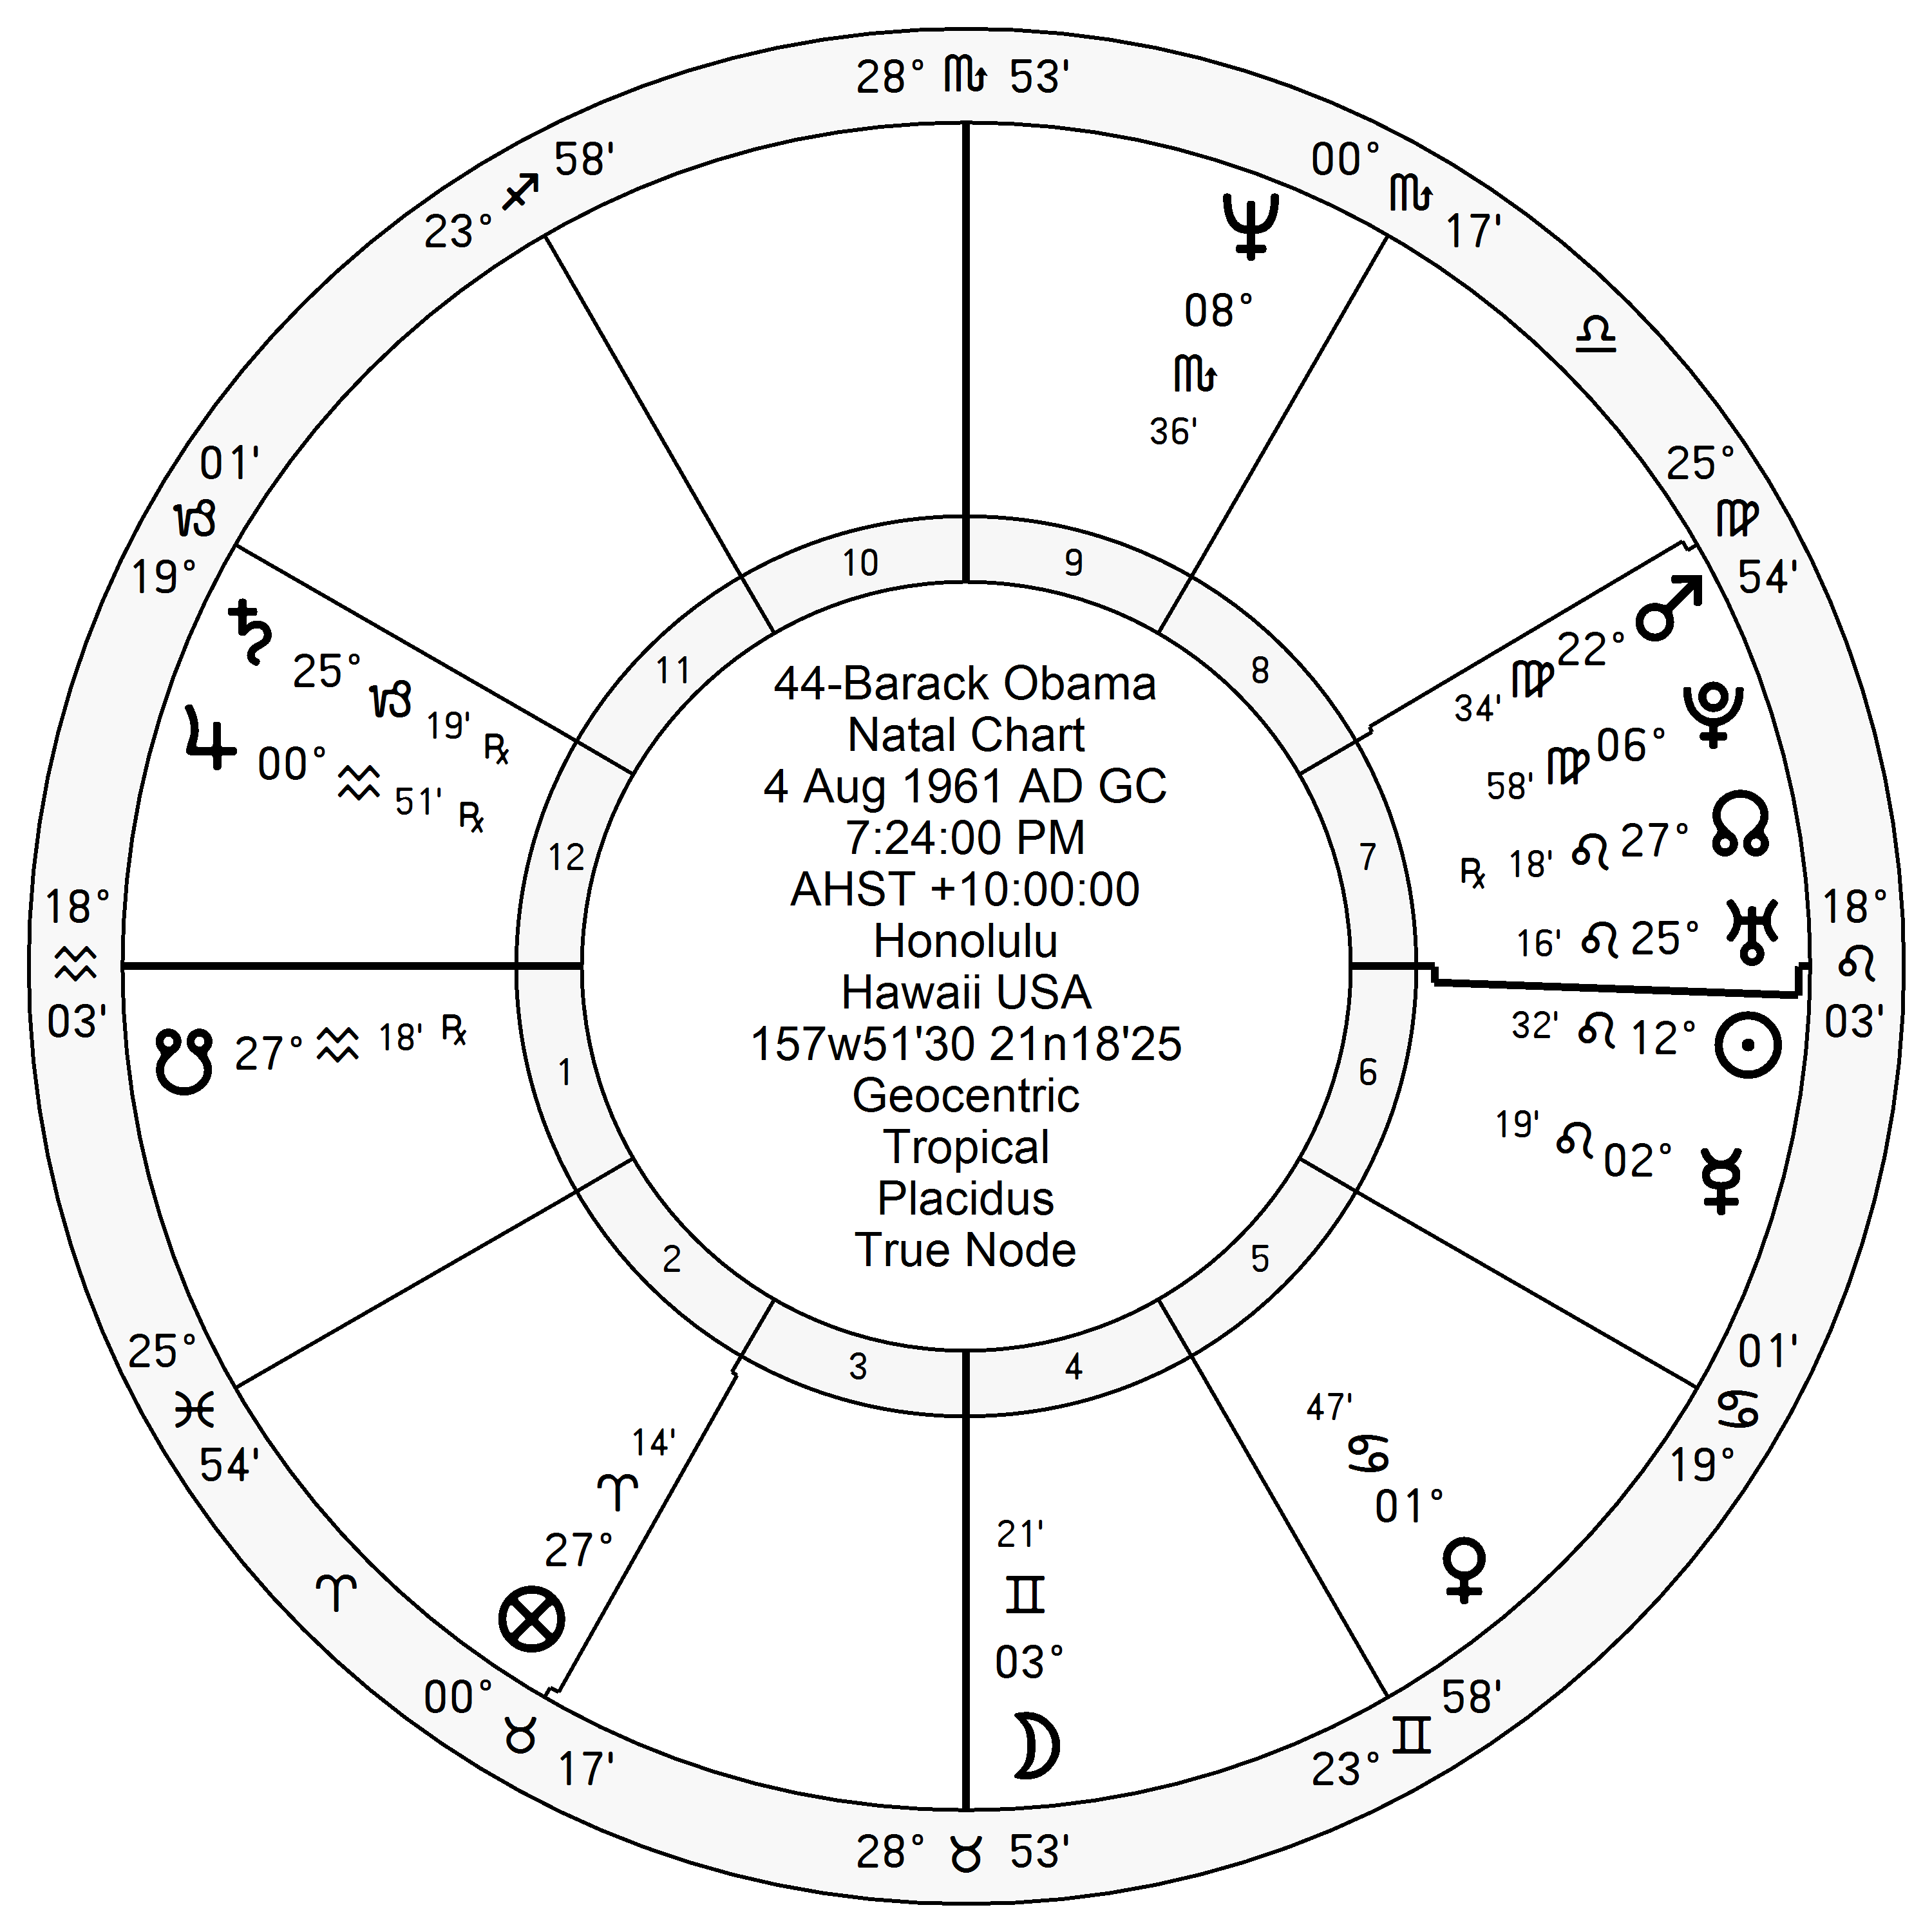
\includegraphics[width=0.9\textwidth]{charts/Obama.png}}
\fontsize{7pt}{8pt}\selectfont

\Venus\, \Trine\, N1; mit. \Quincunx\, (\Opposition) N10 \\
\Saturn\, \Trine\, P1, \Sextile\, N10 \\
\Moon\, in P1 \Square\, P10; \Opposition\, N10, \Square\, N1 \\
\vspace{0.5em}
\SouthNode\, in P10 appeared not to harm him; possibly because Romney had no aspects involving P10 or N10.

\column{0.48\textwidth}
\vspace{-1em}
{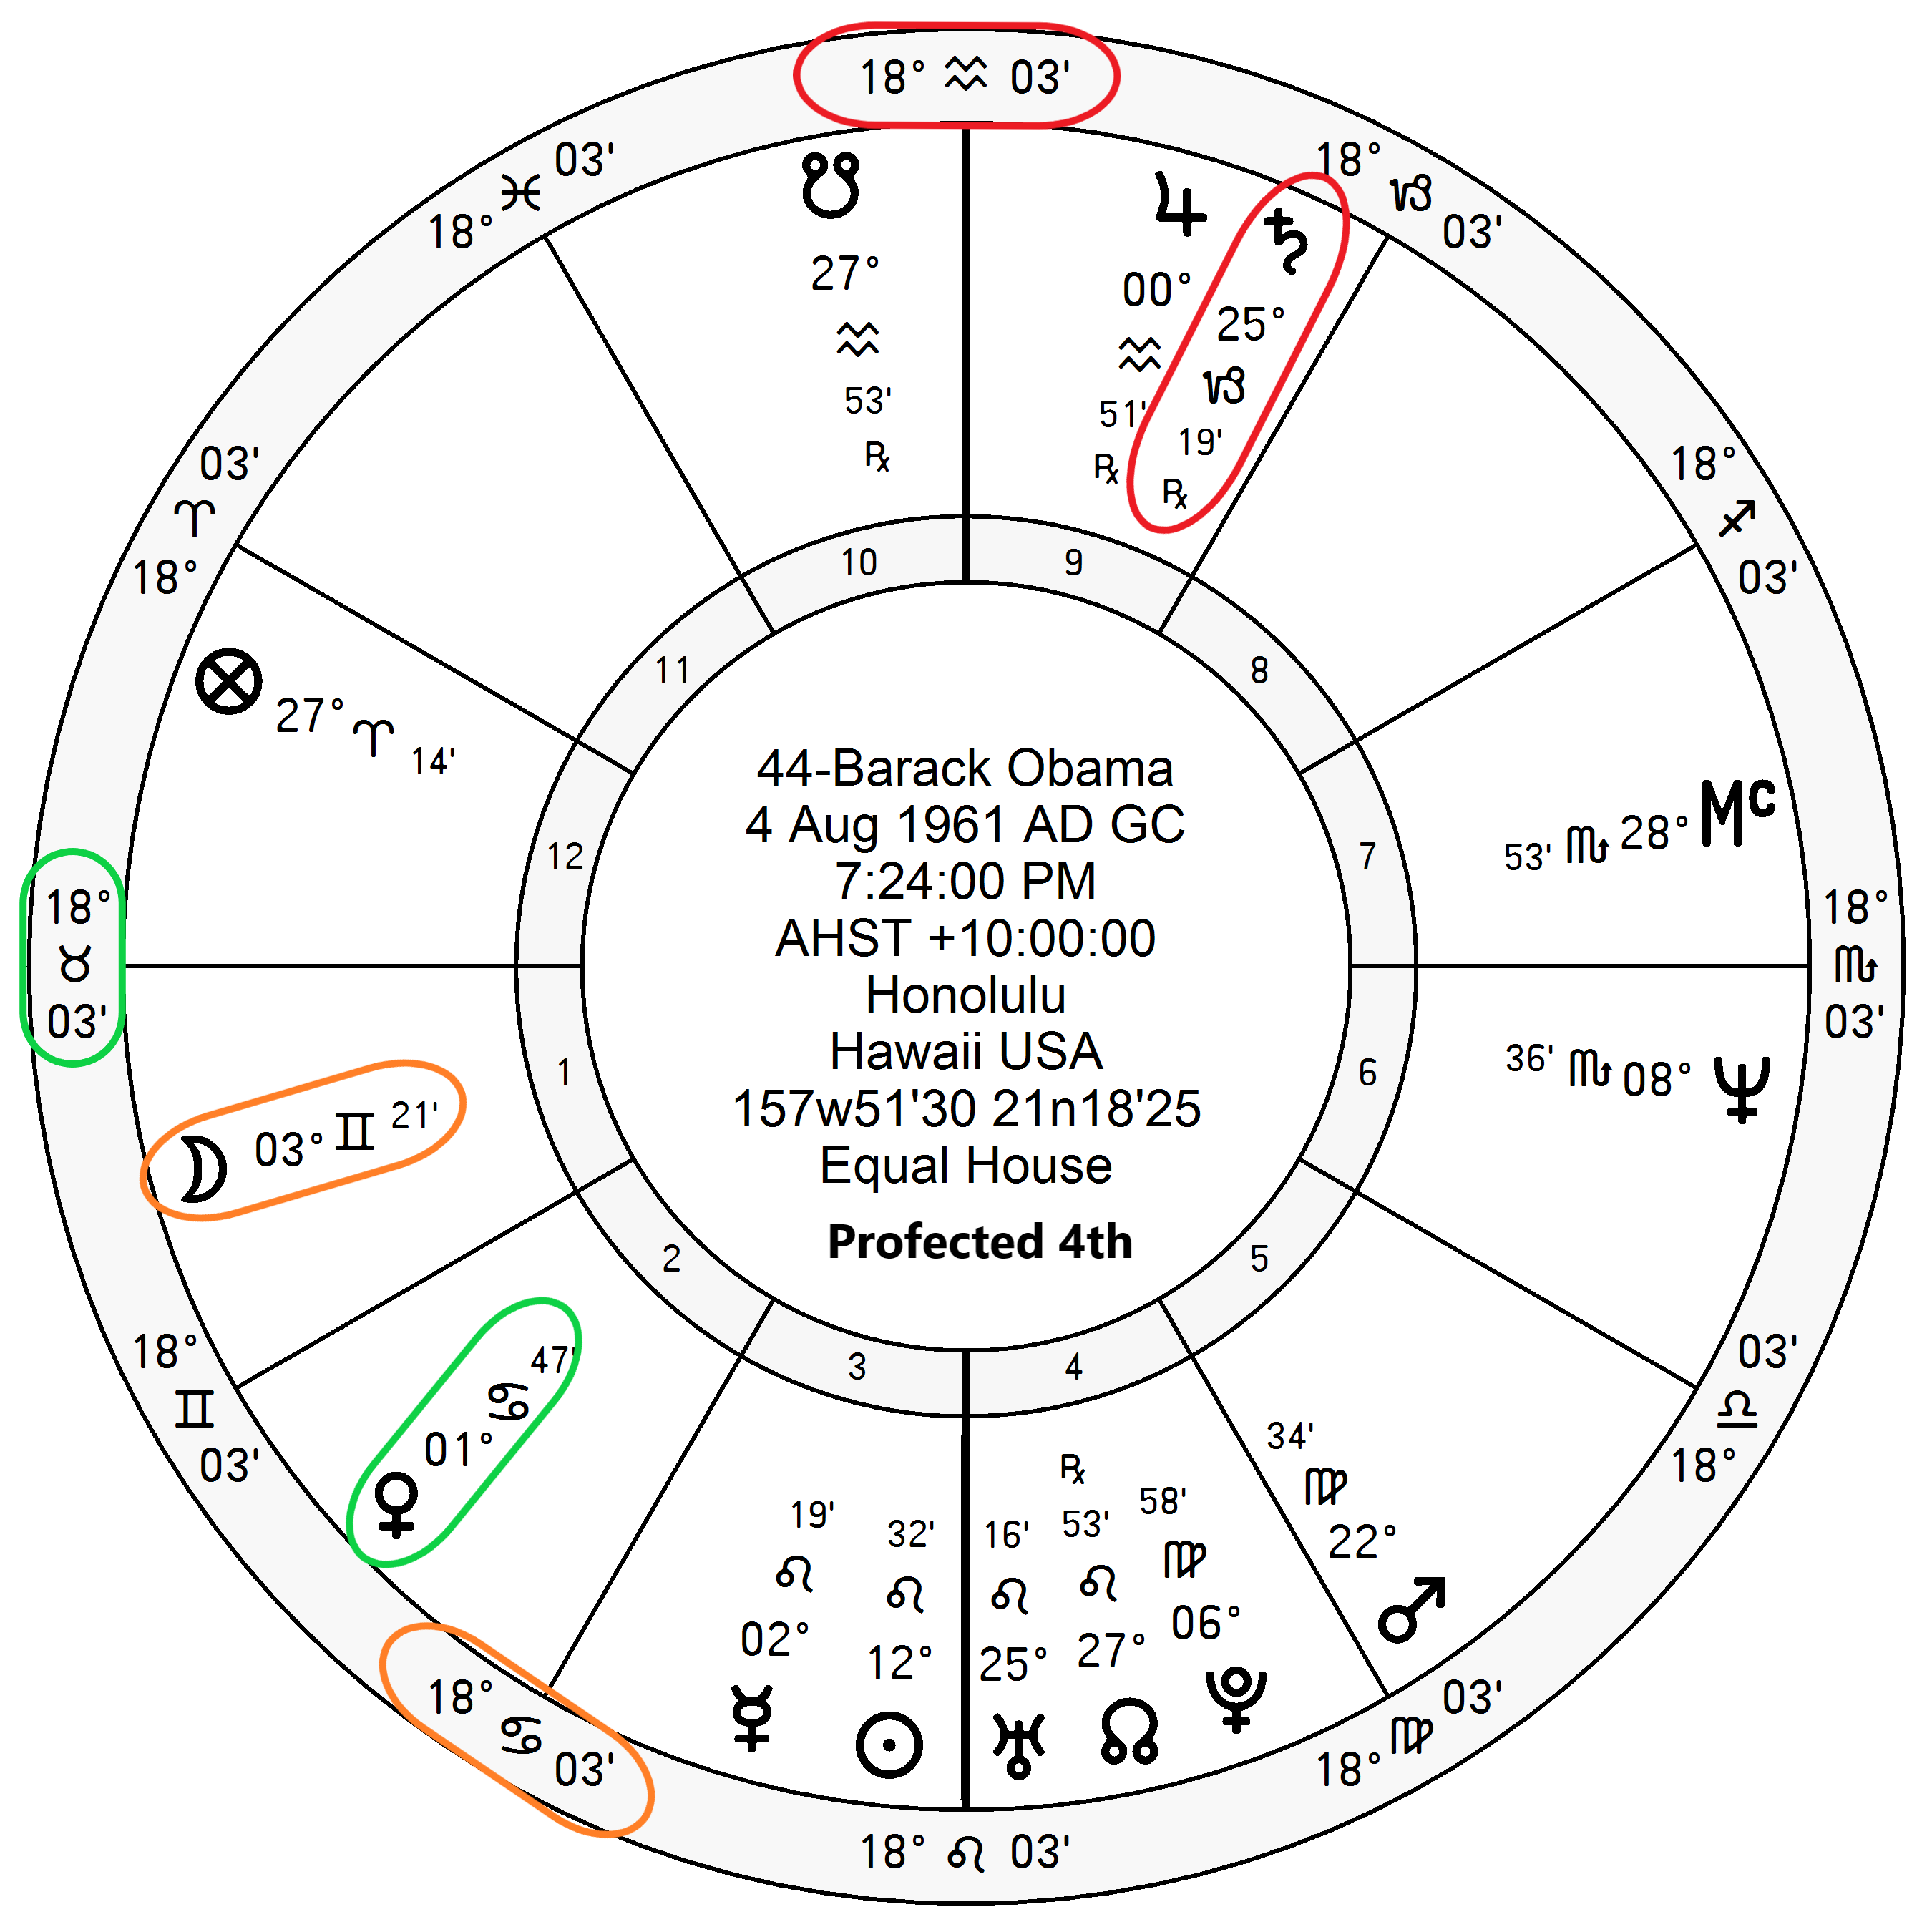
\includegraphics[width=0.9\textwidth]{charts/Obama-Prof-4th.png}}
\fontsize{8pt}{9pt}\selectfont

\textbf{\dgreen P1=N4}
	$\Rightarrow$ \Venus\, $\Rightarrow$ P2/N5\\
\textbf{\red P10}=\textbf{\dgreen N1}
	$\Rightarrow$ \Saturn\, $\Rightarrow$ P9/N12\\
PE=P3/N6
	 $\Rightarrow$ \Moon\, $\Rightarrow$ \textbf{\dgreen P1/N4}

\end{columns}
\end{frame}

% ===================================================
\begin{frame}[t]{Election November 6, 2012: Mitt Romney}
\small
\begin{columns}[T, onlytextwidth]
\column{0.48\textwidth}
\vspace{-1em}
{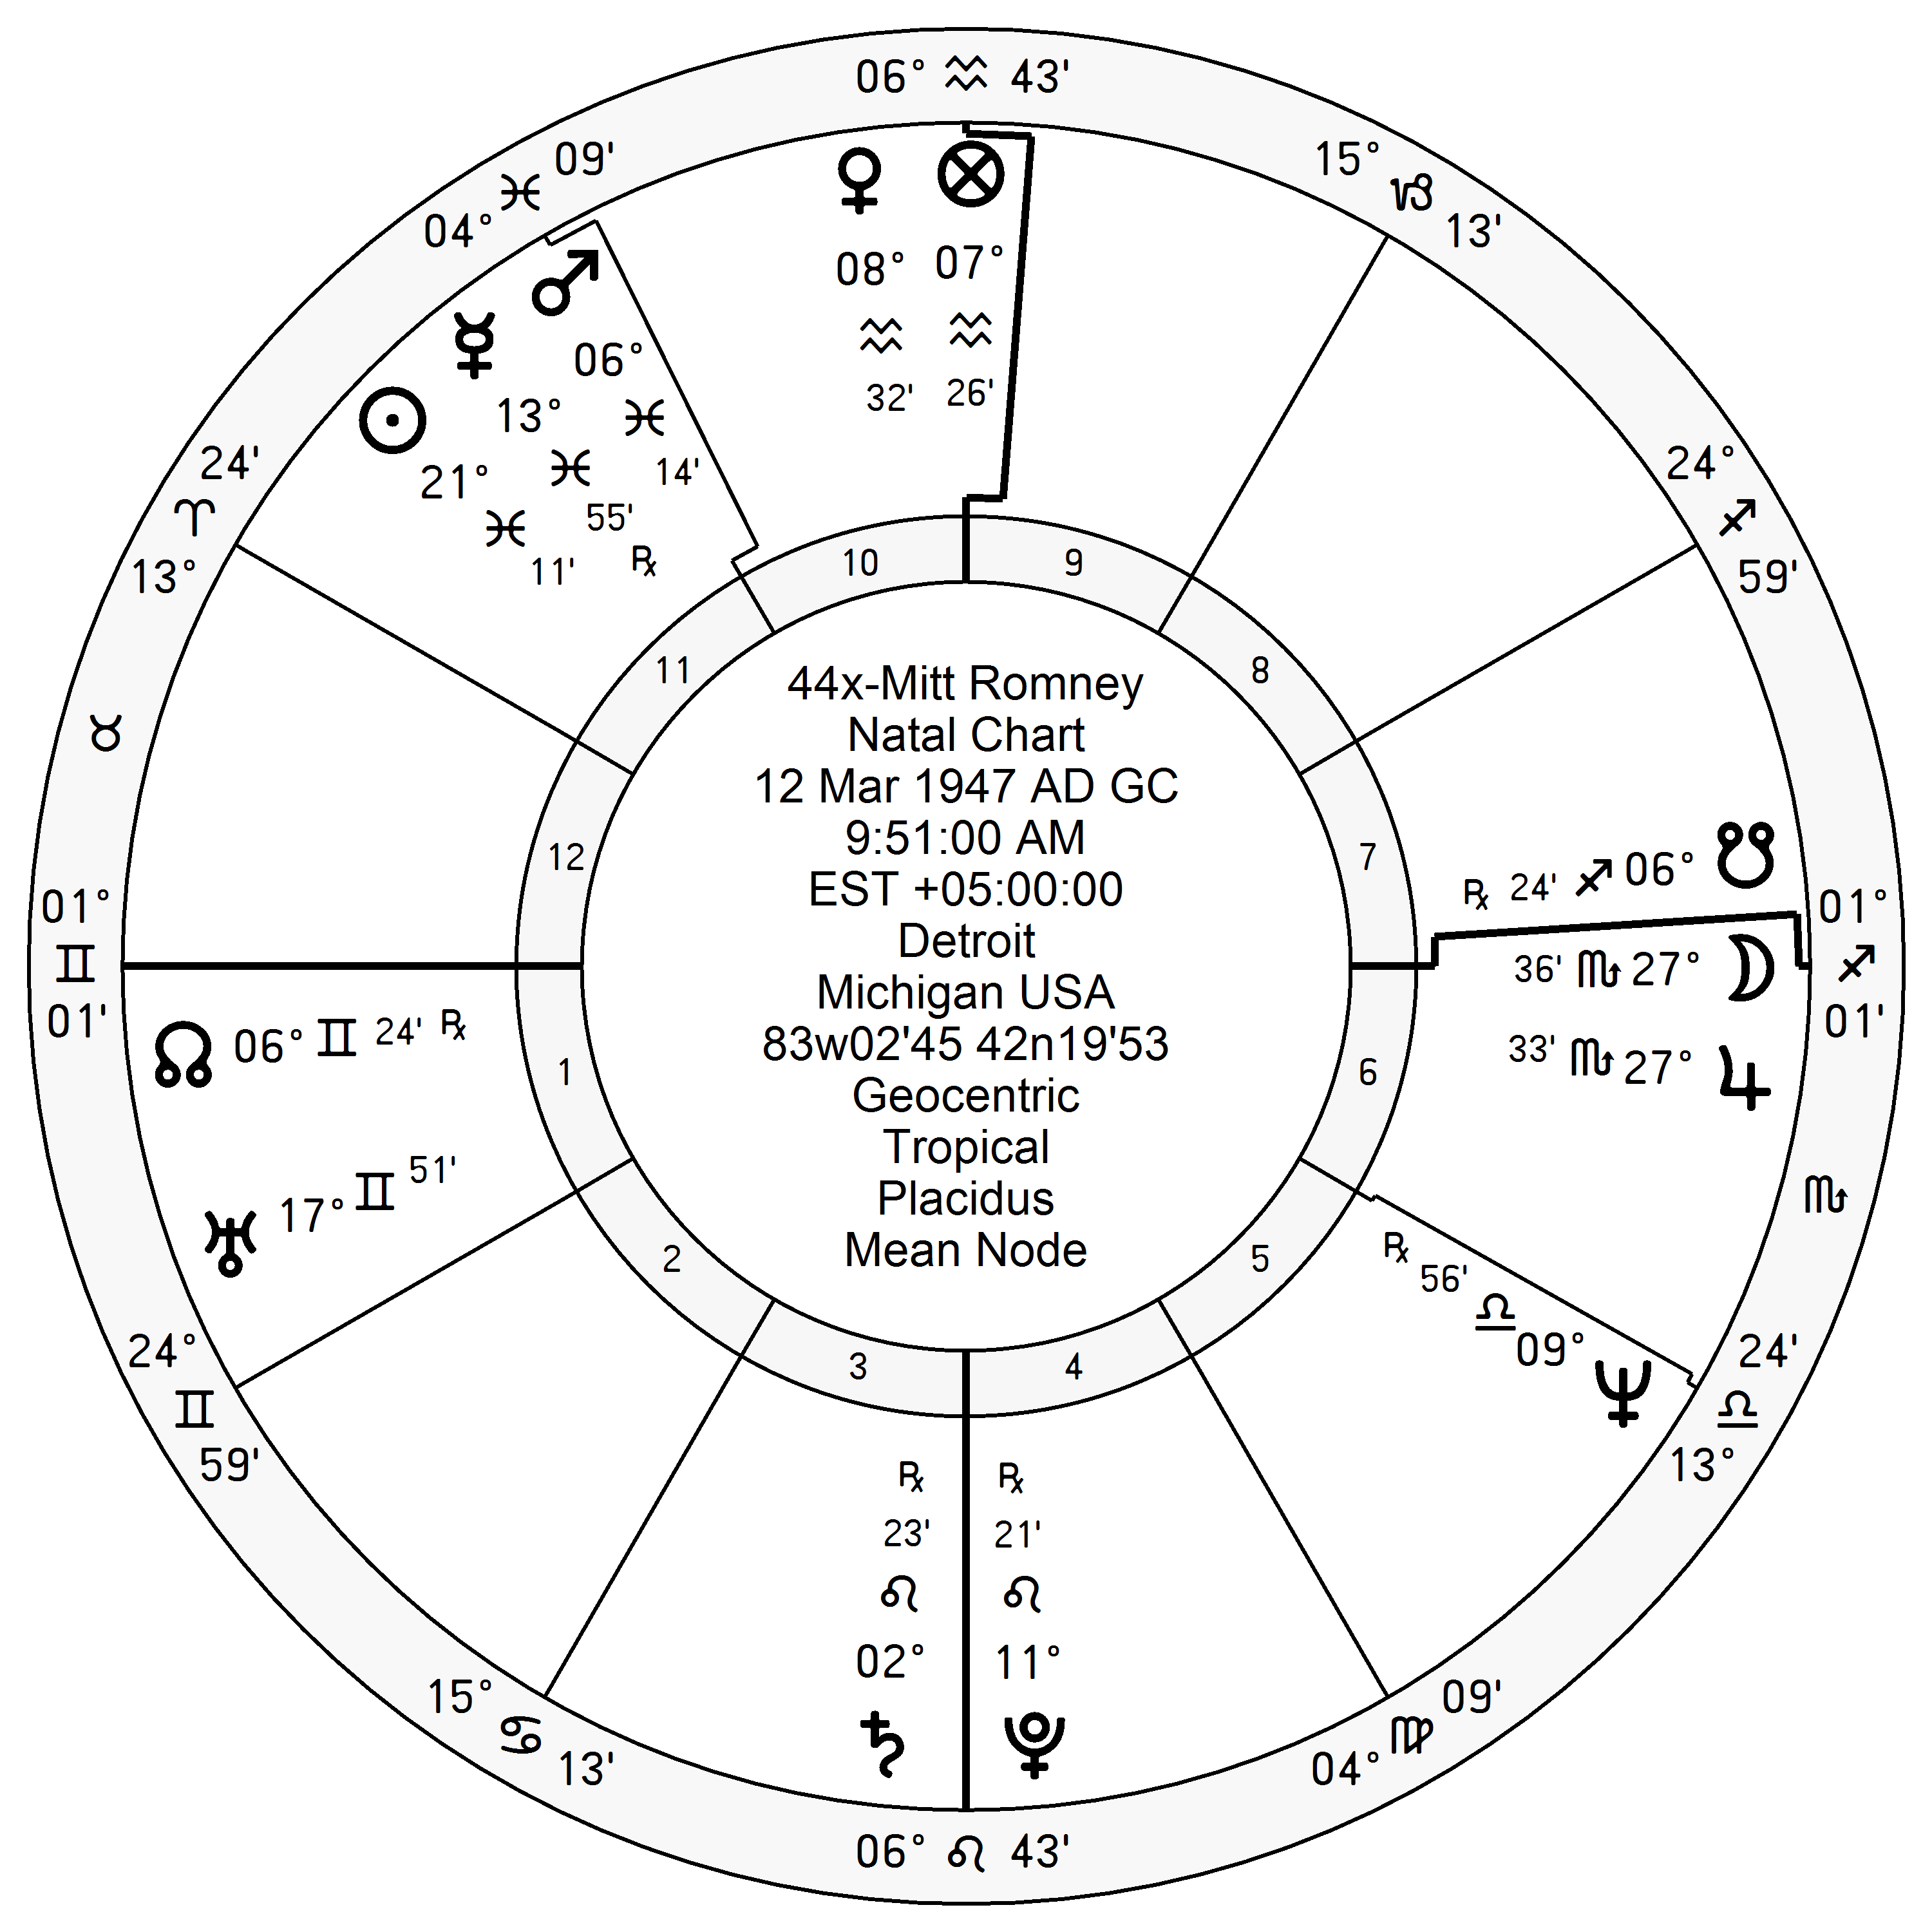
\includegraphics[width=0.9\textwidth]{charts/Romney.png}}
\fontsize{7pt}{8pt}\selectfont

\Mars\, \Trine\, P1; \Square\, N1 \\
\Sun\, \Trine\, P1; \Square\, N1 \\
\Mercury\, burnt \Trine\, P1; \Square\, N1


\column{0.48\textwidth}
\vspace{-1em}
{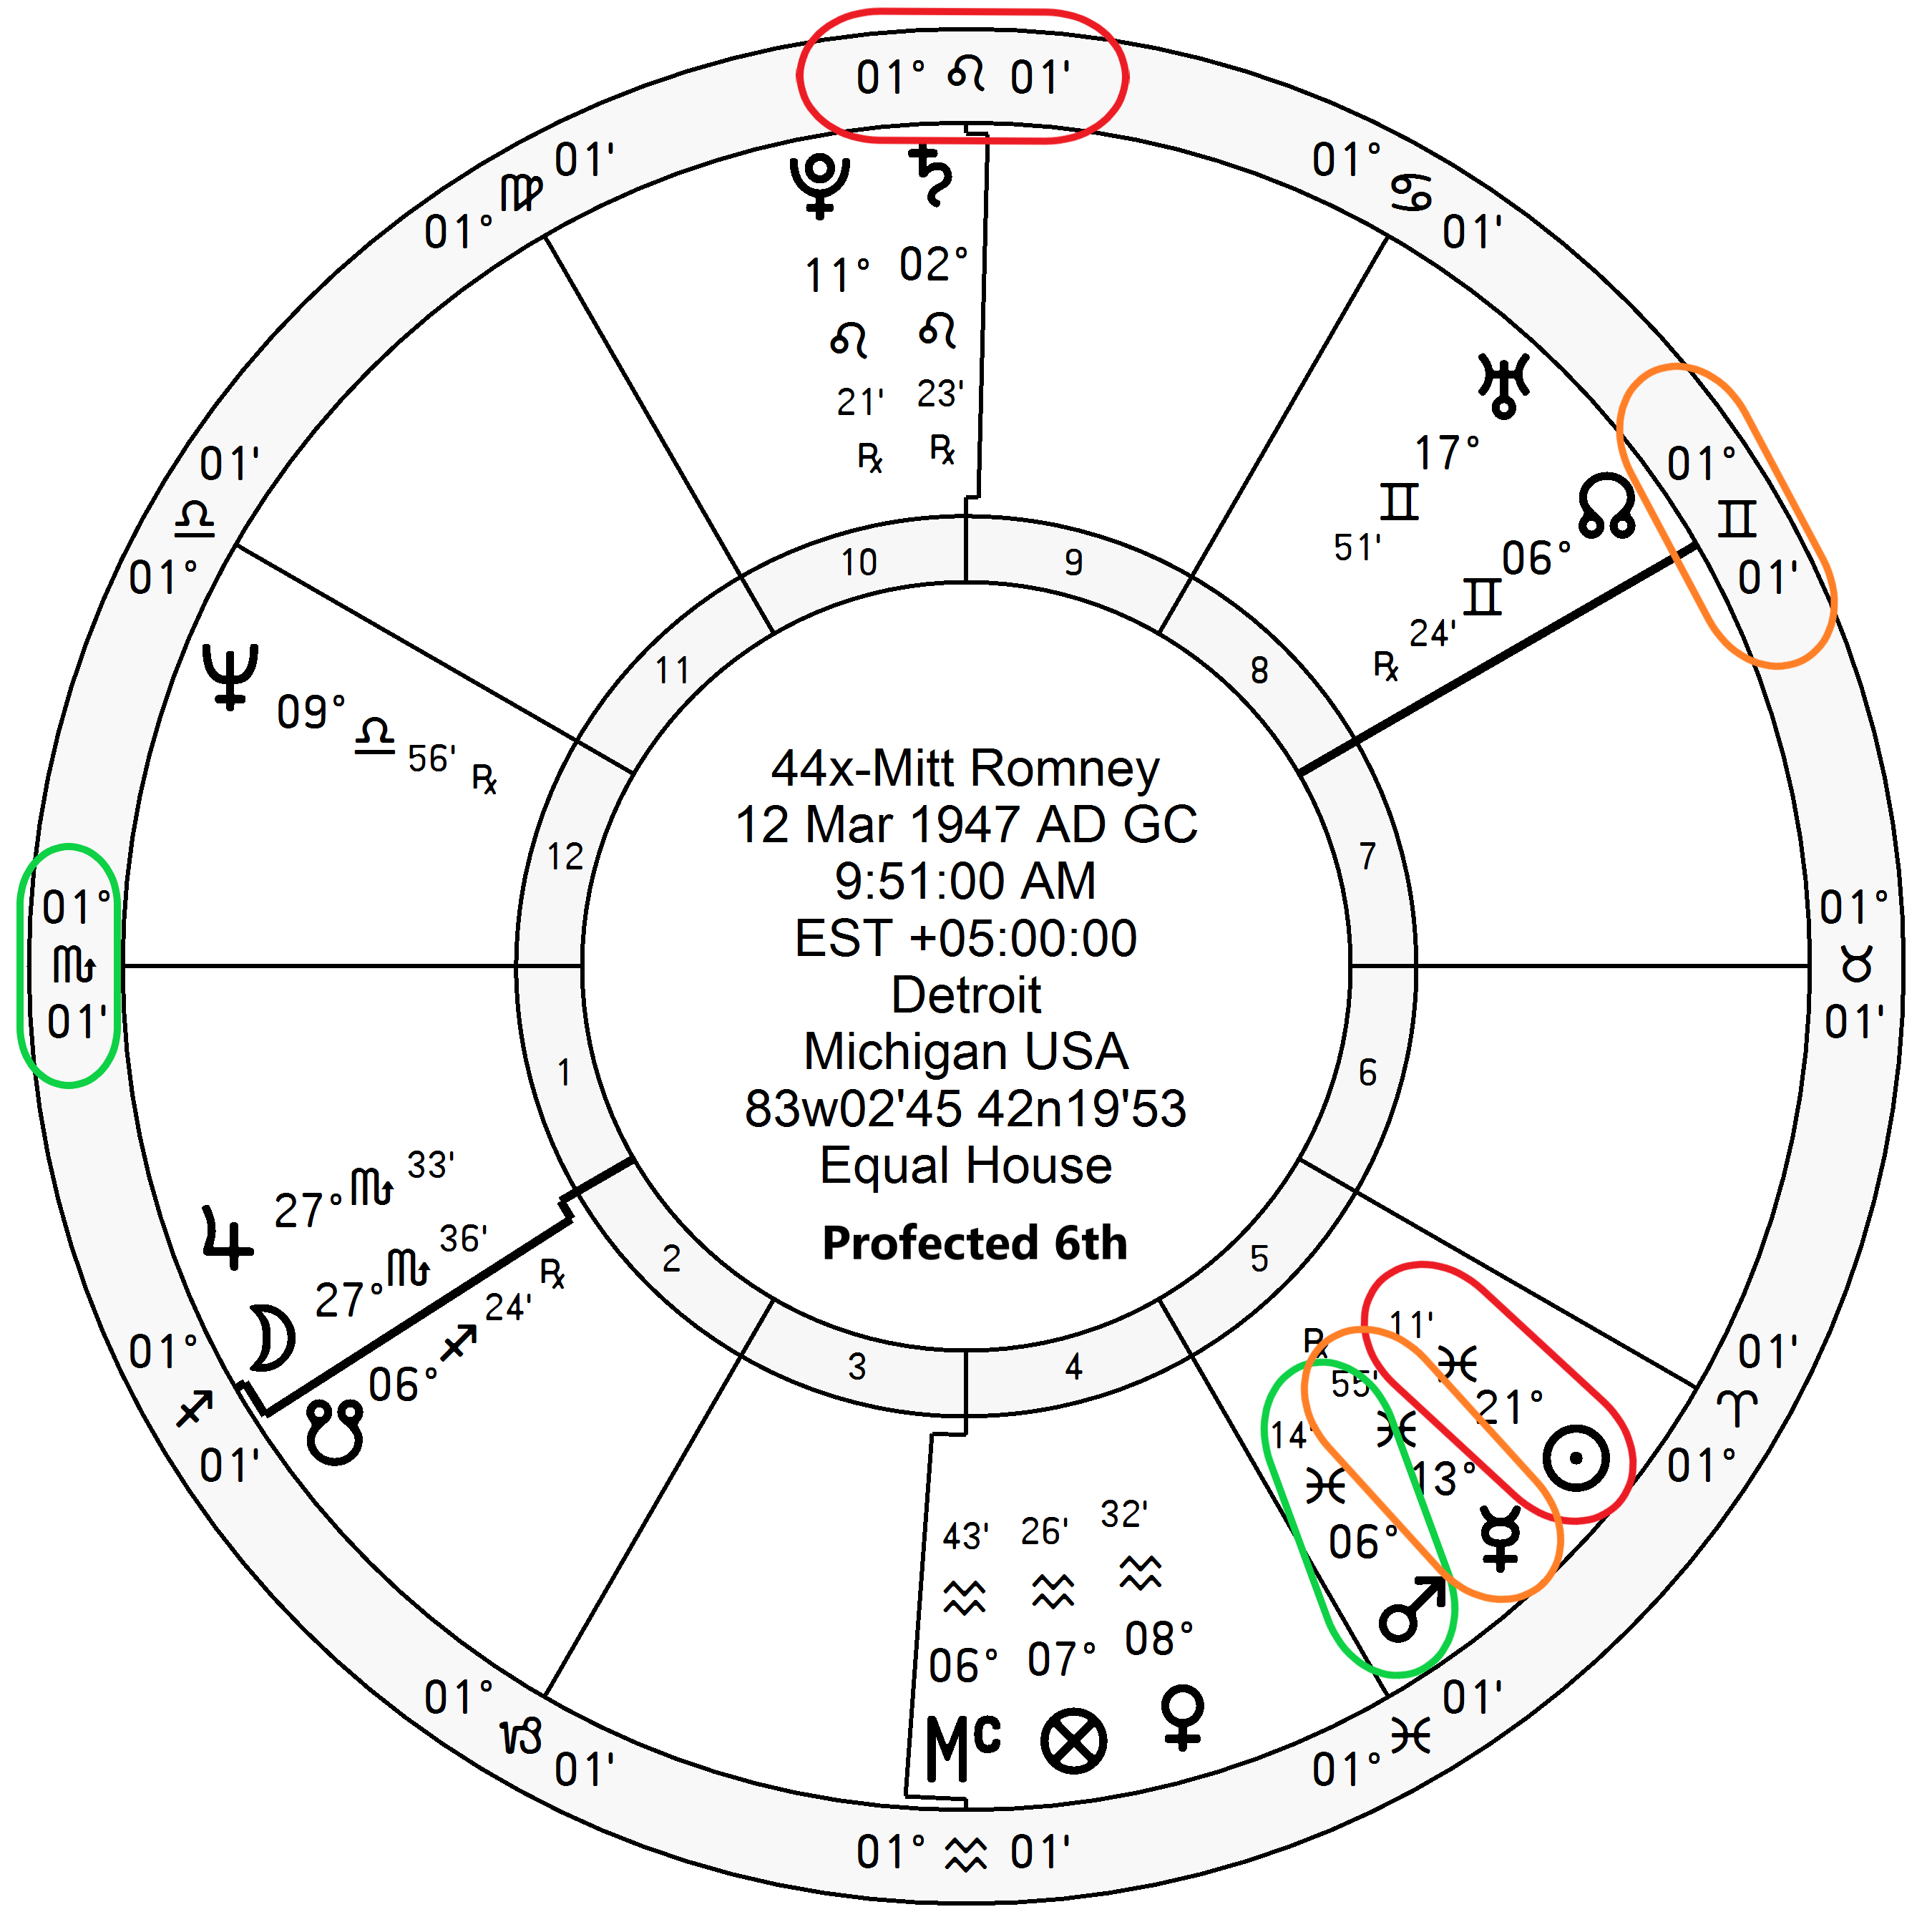
\includegraphics[width=0.9\textwidth]{charts/Romney-Prof-6th.png}}
\fontsize{8pt}{9pt}\selectfont
\textbf{\dgreen P1}=N6
	$\Rightarrow$ \Mars\, $\Rightarrow$ \textbf{\dgreen P5/N11}\\
\textbf{\red P10}=N4
	$\Rightarrow$ \Sun\, $\Rightarrow$ \textbf{\dgreen P5/N11}\\
PE=P8/N2
	 $\Rightarrow$ \Mercury\, $\Rightarrow$ \textbf{\dgreen P5/N11}

\end{columns}
\end{frame}
